\chapter{Konzept und Systemdesign}
\printmyminitoc{1}

In diesem Kapitel wird das Konzept und das Systemdesign für die Arbeit vorgestellt. Insgesamt soll das Forschungsschiff durch einen Spielecontroller
gesteuert werden. Dafür soll ein Rogue Device entwickelt werden, welches in der Lage ist, die Kommunikation des Schiffes zu manipulieren. 
Das Rogue Device soll dabei unbemerkt in das System integriert werden und auf den CAN-Bus für die Motorsteuerung zugreifen. Darauf sollen
manipulierte Steuerbefehle gesendet werden, um den Motor zu steuern. Zusätzlich soll auf den Autopiloten zugegriffen werden, um darüber die Rudersteuerung
zu manipulieren. \\

\section{Aufbau Schiffsysteme}
Ein Schiff besteht aus vielen verschiedenen Systemen, welche verschiedene Aufgaben haben. In diesem Fall wird die
Steuerung des Schiffes betrachtet. Dabei sind die wichtigsten Systeme die Gashebel und die Rudersteuerung, welche den Autopiloten enschließt.
\begin{figure}[H]
    \centering
    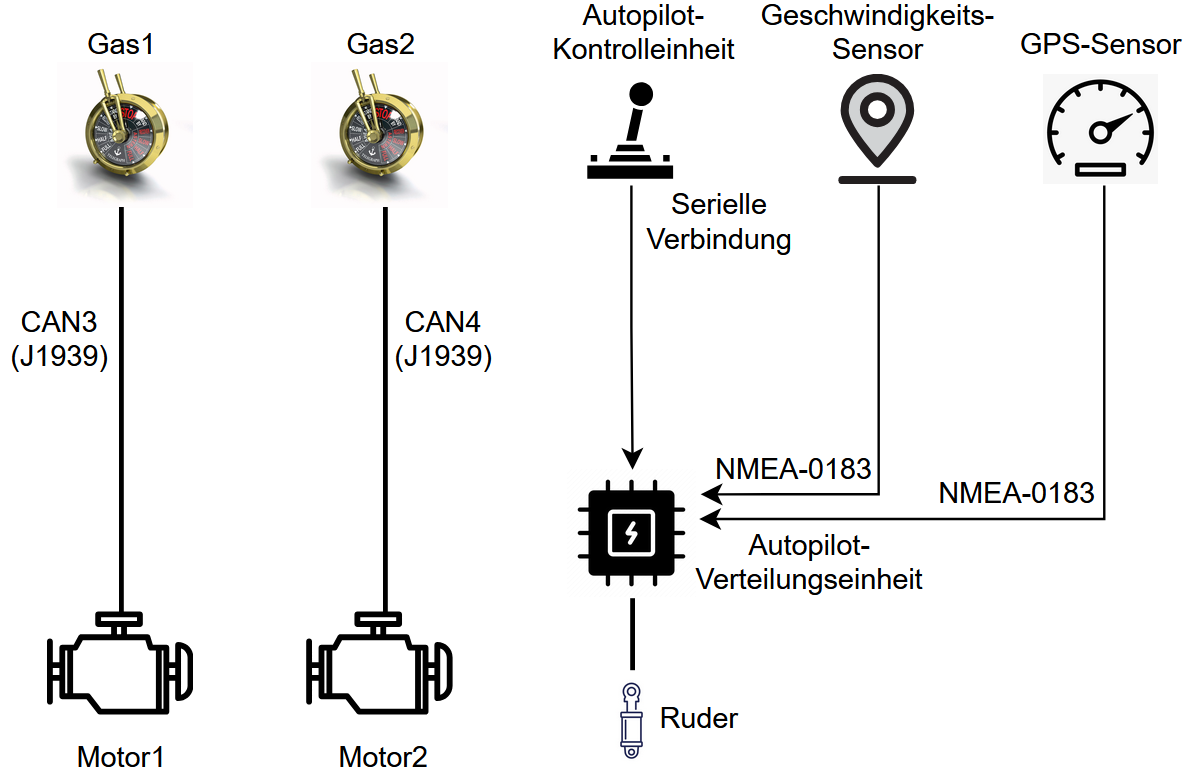
\includegraphics[scale=0.5]{images/limandaSystem.png}
    \caption{Vereinfachte Darstellung der Systeme auf der Limanda}
    \label{fig:limandaSystem}
\end{figure}
In \ref{fig:limandaSystem} sind die genannten Systeme veranschaulicht. Die beiden Gashebel sind jeweils
mit einem CAN-Bus verbunden. Über diese Bussen senden die Gashebel Steuerbefehle an die Motoren. Als Higher-Layer-Protokoll wird J1939 genutzt. \\
Der Autopilot ist ein eigenständiges System, das über eine serielle Schnittstelle mit einer elektronischen Kontrolleinheit(ECU) 
für die Rudersteuerung verbunden ist.
Dieser hat keine Verbindung zu den Gashebeln oder Motoren. Er kann lediglich Signale an die ECU für die Rudersteuerung über
eine serielle Verbindung senden. Die Rudersteuerung ist mit dem Ruderstellmotor über eine unbekannte Verbindung angeschlossen. Diese Verbindung ist
jedoch nicht relevant für diese Arbeit. Für die Kursberechnung erhält der Autopilot Daten von unter anderem einem GPS-Modul und Geschwindigkeitssensor.
Diese Daten werden über NMEA-0183 Nachrichten übertragen. 

\section{Steuerungslogik des Spiele-Controllers} \label{sec:steuerungslogik}
Der benutzte Spiele-Controller ist ein Xbox Series X Controller. Dieser wurde gewählt, da er kabellos ist und kann somit frei bewegt werden. 
Um die Steuerung des Schiffes zu
ermöglichen, müssen die Eingaben des Xbox-Controllers in Steuerbefehle umgewandelt werden. Dies passiert auf dem 
Raspberry Pi. Der Xbox-Controller wird über Bluetooth mit dem Raspberry Pi verbunden. Dort werden die Eingaben des Controllers
ausgelesen und in einem Python-Programm in Steuerbefehle umgewandelt. \\
Um eine einfache Steuerung zu ermöglichen, wird im folgenden die Tastenbelegung aufgeschlüsselt.
Um alle gewünschten Funktionen umzusetzen, werden nicht alle Tasten benötigt. 

\begin{figure}[H]
    \centering
    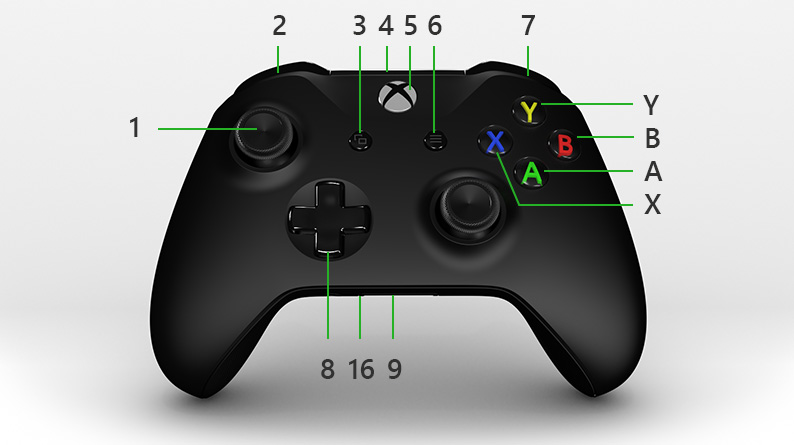
\includegraphics[scale=0.5]{images/vorderseite.jpg}
    \caption{Vorderseite des Xbox-Controllers \cite{XboxController}}
    \label{fig:vorderseite}
\end{figure}

\begin{figure}[H]
    \centering
    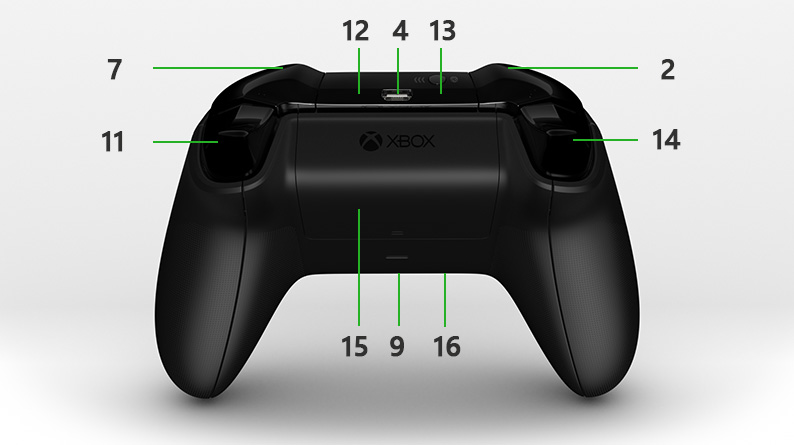
\includegraphics[scale=0.5]{images/rueckseite.jpg}
    \caption{Rückseite des Xbox-Controllers \cite{XboxController}}
    \label{fig:rueckseite}
\end{figure}

In den Abbildungen \ref{fig:vorderseite} und \ref{fig:rueckseite} sind die Tasten des Xbox-Controllers zu sehen.
Die Tastenbelegung ist wie folgt:

\begin{table}[H]
    \begin{tabular}{|c|c|}
    \hline
    \rowcolor[gray]{0.8}
     Nummerierung der Taste & Funktion \\ \hline 
     1 & Bewegung des Ruders \\ \hline 
     2 & Reduzierung der linken Gashebelposition \\ \hline 
     7 & Reduzierung der rechten Gashebelposition \\ \hline
     11 & Erhöhung der rechten Gashebelposition \\ \hline
     14 & Erhöhung der linken Gashebelposition \\ \hline
     B + 2 & Umschalten des Rückwärtsgangs am linken Motor \\ \hline
     B + 7 & Umschalten des Rückwärtsgangs am rechten Motor \\ \hline
     B + 2 + 7 & Umschalten des Rückwärtsgangs an beiden Motoren \\
      & (basierend auf dem derzeitigen Gang am rechten Motor) \\ \hline
    \end{tabular}
\end{table}
Das Einlegen des Rückwärtsgangs ist durch eine Tastenkombination so gewählt, dass es nicht aus Versehen passieren kann.
Mit jeweils der Taste 2 oder 7 wird die Gashebelposition reduziert. Mit der zusätzlichen Betätigung der Taste B wird der 
Rückwärtsgang eingelegt an dem jeweiligen Motor. Wenn die Tasten 2, 7 und B gleichzeitig betätigt werden, 
wird der Rückwärtsgang für beide Motoren gleichzeitig umgeschaltet.
Damit das Getriebe während des Schaltvorgangs keine Gaseingabe erhält und möglicherweise Schaden nimmt, 
ist eine Verzögerung von 10 Sekunden eingebaut. 
Das soll dem Getriebe genug Zeit geben, um den Gang zu wechseln.
Allerdings soll es auch eine Möglichkeit geben, beide Getriebe gleichzeitig umzuschalten, um nicht 
nacheinander die Verzögerung zu haben. Dies wird durch die Tastenkombination B + 2 + 7 realisiert.
Dabei wird der Gang des rechten Motors als Referenz genommen. \\

\section{Integration des Rogue Device}
Damit der Controller die Steuerbefehle an das Schiff senden kann, muss das Rogue Device in das System integriert werden.
In diesem Fall ist das Rogue Device der Raspberry Pi. Damit dieser möglichst unbemerkt in das System integriert werden kann,
muss der Controller drahtlos verbunden werden. Zusätzlich muss das Rogue Device auch mit Strom versorgt werden. 
Dafür könnte ein Akku genutzt werden. Dieser müsste jedoch regelmäßig geladen werden. Daher ist es sinnvoller, die Stromversorgung
über das Schiff zu realisieren. 
 \\
Um die Kommunikation von dem Rogue Device zu dem Schiff zu ermöglichen, müssen
die einzelnen Systeme angesteuert werden. Um die Gashebelposition zu verändern, wird der Raspberry Pi mit dem CAN-Bus des Schiffes
verbunden. \\
Der Spiele-Controller soll über Bluetooth mit dem Raspberry Pi verbunden. Dieser liest die Eingaben des Controllers aus und
übersetzt die in entsprechende Nachrichten. Daraufhin werden die Nachrichten an den CAN-Bus und an die Rudersteuerung gesendet.

\subsection{Manipulation des Gashebels}
Die Manipulation des Gashebels soll durch manipulierte Nachrichten auf dem CAN-Bus realisiert werden.
Das Rogue Device wird dazu als externes Gerät an den CAN-Bus angeschlossen. Der Gashebel bleibt weiterhin angeschlossen.
Sollte der Gashebel in der normalen Benutzung vom Schiffsführer benutzt werden, wird ein Signal an den CAN-Bus gesendet. 
Dieses Signal wird dann an die Motoren weitergeleitet. Wenn das Rogue Device keine Nachricht sendet, kann es durchaus sein, dass
die der Gashebel die Befehle überschreibt.
Um echte Eingaben zu verhindern, muss auf diese Nachricht erkannt und darauf reagiert werden. 
Dazu muss ein Programm auf dem Rogue Device die Nachrichten auf dem CAN-Bus abhören und analysieren.
Wenn eine Nachricht für die Motorsteuerung erkannt wird, kann eine Nachricht des Rogue Device gesendet werden, um die Gashebelposition
zu überschreiben. 
Da die manipulierten Nachrichten dem gleichen Typ entsprechen, wie die echten Nachrichten, ist es wichtig, die eigenen Nachrichten
unterscheiden zu können.
Das muss geschehen, um eine Endlosschleife von eigenen Nachrichten zu verhindern. Dafür könnte
der Nachrichtenzähler überwacht werden. Aus den aufgezeichneten Nachrichten hat sich herausgestellt, dass der 
Nachrichtenzähler wenige verschiedene Werte hat. Daher sind diese Werte zu den eigenen erstellten Nachrichten 
verschieden. Dies ist eine einfache Methode, um die eigenen Nachrichten zu erkennen. Eine bessere Möglichkeit ist es aber,
eine eigene CAN-ID zu berechnen. Diese kann dann genutzt werden, um die eigenen Nachrichten zu erkennen. \\
Wie in der Abbildung \ref{fig:j1939header} zu sehen, besteht der Header aus einer PGN, einer Quelladresse und einer Priorität. Um nun Nachrichten
an den Motor zu senden, kann eine Nachricht des Gashebels abgefangen werden. Die PGN kann für die eigene Nachricht genutzt
werden. Die Quelladresse kann auch kopiert werden. Die Priorität sollte möglichst klein gewählt werden, 
damit die Nachricht des Rogue Devices bevorzugt wird. In der eigenen Nachricht kann dann die gewünschte Gashebelposition gesendet werden.

\subsection{Manipulation der Rudersteuerung}
Um die Rudersteuerung zu manipulieren, muss der Raspberry Pi mit dem Autopiloten verbunden werden. Bei dem Autopiloten
handelt es sich um ein Navitron NT888G. Die Eingabeeinheit ist über eine serielle Schnittstelle mit einer elektronischen Kontrolleinheit. 
Diese Verbindung ist unverschlüsselt, benutzt jedoch ein Proprietäres Protokoll von Navitron.
Durch Reverse-Engineering müssen einzelne Befehle herausgefunden werden, welche für die Ruderkontrolle von Bedeutung sind.
Dazu müssen die Nachrichten des Autopiloten abgefangen und analysiert werden. Mit den gewonnenen Informationen können
eigene Nachrichten erstellt werden oder bestehende Nachrichten in eigener Reihenfolge abgespielt werden.
Zusätzlich kann das Ruder auch physikalisch über das Steuerrad bewegt werden. Dieser Weg wird jedoch nicht betrachtet.
Ein weiterer Ansatz wäre es, die echten Kursdaten abzufangen und zu manipulieren. Dadurch müsste der Autopilot reagieren
und das Ruder steuern. Die Kursdaten werden nach dem NMEA-0183-Standard gesendet. \\
Aufgrund des Alters dieses Standards sind Informationen über das Format der Nachrichten verfügbar. Damit können die Kursdaten
einfach verstanden und manipuliert werden. Mit dem Austauschen der echten Daten durch manipulierte, wäre ein 
physikalischer Man-in-the-Middle Angriff realisiert.\\

\subsection{Rückmeldung der Eingaben}
Es muss eine Art der Rückmeldung für den 'Angreifer' geben, um in etwa die Eingaben im Vergleich zum momentanen Zustand zu sehen.
Dabei sollte die Rückmeldung möglichst unauffällig sein. Ein kleiner Bildschirm könnte benutzt werden, dieser kann 
physisch an den Raspberry Pi angeschlossen werden. Das würde das Verstecken des Rogue Devices erschweren.
Ein eigenständiges Display könnte auch über eine Funkttechnologie mit dem Raspberry Pi verbunden werden.
Eine andere Möglichkeit stellt eine App auf einem Handy dar. Diese App könnte dann die gewünschten Positionen anzeigen.
Dafür muss der Raspberry Pi mit dem Handy verbunden werden. Dies könnte über Bluetooth geschehen.
Hier ist zu beachten, dass die Verbindung stabil sein muss und nicht von anderen Geräten gestört wird.
Jedoch kann ist hier mit einem größeren Aufwand zu rechnen, da die App erst entwickelt werden muss.
Eine weitere Möglichkeit würden Vibrationen im Xbox Controller sein. Diese könnten genutzt werden, wenn die derzeitige
Eingabe ein Maximum oder Minimum erreicht hat. Allerdings ist dies nicht so genau wie eine Anzeige auf einem Bildschirm.
Es könnten auch nur wenige bestimmte Positionen mittgeteilt werden. \\
Eine solche Rückmeldung ist wichtig, um die Eingaben zu überprüfen und gegebenenfalls anzupassen.
Da die Steuerung auf einem Schiff generell Trägheit aufweist, ist es wichtig, die Eingaben frühzeitig zu korrigieren.
Daher können Änderungen in den Eingaben nicht sofort sichtbar sein. Es muss also eine Möglichkeit geben, die Eingaben
zu überprüfen.